% Reporte de la actividad 4A — Buscador semántico híbrido y re-ranking con Transformers
% Compilación: latexmk -pdf -jobname=Reporte_Actividad4A reporte.tex
% Las cifras provienen de results/*.csv y las figuras de figures/ (generadas por el notebook).
% Límite de la actividad: máximo tres páginas.
\documentclass[10pt,a4paper]{article}

\usepackage[T1]{fontenc}
\usepackage[utf8]{inputenc}
\usepackage[spanish,es-nodecimaldot]{babel}
\usepackage[margin=1.7cm,top=1.5cm,bottom=1.6cm]{geometry}
\usepackage{amsmath}
\usepackage{booktabs}
\usepackage{array}
\usepackage{xcolor}
\usepackage{microtype}
\usepackage{enumitem}
\usepackage{graphicx}
\usepackage{float}
\usepackage[font=small,labelfont=bf,skip=2pt]{caption}
\usepackage[hidelinks]{hyperref}

\graphicspath{{figures/}}

\definecolor{acento}{HTML}{1F6FEB}
\newcommand{\term}[1]{\textcolor{acento}{\texttt{#1}}}
\newcommand{\q}[1]{\emph{«#1»}}

\setlist[itemize]{topsep=1pt,itemsep=0pt,parsep=0pt,leftmargin=1.2em}
\setlist[enumerate]{topsep=1pt,itemsep=0pt,parsep=0pt,leftmargin=1.5em}
\setlength{\parskip}{2pt}
\setlength{\textfloatsep}{6pt}
\setlength{\floatsep}{6pt}
\setlength{\intextsep}{5pt}
\renewcommand{\arraystretch}{1.02}
\usepackage{titlesec}
\titlespacing*{\section}{0pt}{5pt}{2pt}
\titlespacing*{\paragraph}{0pt}{3pt}{0.6em}

\title{\vspace{-1.5cm}\textbf{Buscador semántico híbrido y \emph{re-ranking} con Transformers}\\[2pt]
\large Qué entiende la recuperación densa que BM25 no, y cuánto cuesta la segunda etapa}
\author{David Segundo García}
\date{\vspace{-0.3cm}Actividad 4A \textperiodcentered\ 26 de octubre de 2026
\textperiodcentered\ acompaña al notebook \texttt{Actividad4A\_Buscador\_Semantico.ipynb}}

\begin{document}
\maketitle
\vspace{-0.9cm}

\section{Sistema y montaje experimental}

\paragraph{Corpus y línea base.} Se reutilizan los \textbf{120 documentos en español} de la unidad 2
(12 temáticas, 45--81 palabras cada uno) y su BM25 ($k_1=1.5$, $b=0.75$, \emph{stemming} Snowball), que
reproduce las puntuaciones de la actividad 2A.

\paragraph{Pipeline de dos etapas.} (1) Un \emph{bi-encoder} codifica cada documento (título + texto)
en un vector unitario. La consulta se codifica con el mismo modelo y un índice \textbf{HNSW}
(\texttt{hnswlib}, el recomendado en la unidad 3) devuelve el \textbf{Top-20 por similitud coseno}. Sobre
las 20 consultas de evaluación, el índice reproduce exactamente el Top-20 de la búsqueda exhaustiva. (2)
Un \emph{cross-encoder} lee cada par consulta--documento completo y reordena esos 20 candidatos.
Se probaron dos modelos en cada etapa:

\begin{table}[H]
\centering\footnotesize\setlength{\tabcolsep}{4pt}
\begin{tabular}{@{}lllrrl@{}}
\toprule
\textbf{Etapa} & \textbf{Clave} & \textbf{Modelo (Hugging Face)} & \textbf{Dim.} & \textbf{Parám.} & \textbf{Entrenamiento} \\
\midrule
\emph{Bi-encoder}    & MiniLM & \texttt{paraphrase-multilingual-MiniLM-L12-v2} & 384 & 118\,M & paráfrasis, 50+ idiomas \\
\emph{Bi-encoder}    & E5     & \texttt{intfloat/multilingual-e5-base}          & 768 & 278\,M & recuperación (prefijos \texttt{query:}/\texttt{passage:}) \\
\emph{Cross-encoder} & mMARCO & \texttt{mmarco-mMiniLMv2-L12-H384-v1}           & --- & 118\,M & MS MARCO traducido a 14 idiomas \\
\emph{Cross-encoder} & BGE    & \texttt{BAAI/bge-reranker-v2-m3}                & --- & 568\,M & \emph{ranking} multilingüe \\
\bottomrule
\end{tabular}
\end{table}

\paragraph{Evaluación.} Se escribieron \textbf{20 consultas}: 8 \emph{léxicas}, que comparten
vocabulario con su documento, y 12 de \emph{paráfrasis}, que usan sinónimos o lenguaje cotidiano. Tienen
48 juicios graduados (2 = muy relevante, 1 = parcial), asignados leyendo los 120 documentos con un
criterio fijo y sin modificarlos después de ver los resultados. Las métricas son \textbf{nDCG@5} (principal, con ganancia $2^{rel}-1$), MRR y
recall@5. Se midió la latencia en CPU (Apple M5, 20 consultas $\times$ 5 repeticiones). Ningún documento
supera el límite de 128 \emph{tokens} de MiniLM, así que ambos modelos ven el texto completo.

\section{Resultados cuantitativos}

\begin{table}[H]
\centering\small
\begin{tabular}{@{}lccccccr@{}}
\toprule
& & & & \multicolumn{2}{c}{\textbf{nDCG@5 por tipo}} & & \\
\cmidrule(lr){5-6}
\textbf{Configuración} & \textbf{nDCG@5} & \textbf{MRR} & \textbf{R@5} & \textbf{léxica} & \textbf{paráfrasis} & \textbf{R@20} & \textbf{ms (mediana)} \\
\midrule
BM25 (unidad 2)              & 0.725 & 0.875 & 0.642 & 0.940 & 0.582 & 0.696 & 0.08 \\
MiniLM (coseno)              & 0.880 & 1.000 & 0.842 & 0.939 & 0.841 & 0.975 & 8.6 \\
E5 (coseno)                  & 0.951 & 1.000 & 0.938 & 0.970 & 0.938 & 0.975 & 20.2 \\
MiniLM + mMARCO              & 0.889 & 1.000 & 0.842 & 0.941 & 0.854 & 0.975 & 189.8 \\
E5 + mMARCO                  & 0.887 & 1.000 & 0.842 & 0.942 & 0.850 & 0.975 & 195.7 \\
MiniLM + BGE                 & \textbf{0.959} & 1.000 & \textbf{0.950} & 0.970 & \textbf{0.951} & 0.975 & 1\,740.0 \\
E5 + BGE                     & \textbf{0.959} & 1.000 & \textbf{0.950} & 0.970 & \textbf{0.951} & 0.975 & 1\,679.1 \\
Híbrido RRF (BM25 + E5)      & 0.857 & 0.950 & 0.850 & \textbf{0.975} & 0.778 & 0.975 & $\approx$20 \\
Híbrido RRF + BGE            & \textbf{0.959} & 1.000 & \textbf{0.950} & 0.970 & \textbf{0.951} & 0.975 & $\approx$1\,680 \\
\bottomrule
\end{tabular}
\caption{Promedios sobre 20 consultas (\texttt{results/metricas\_por\_configuracion.csv}). R@20 es el
techo de la primera etapa: el \emph{re-ranking} solo reordena lo que recibe.}
\end{table}

\begin{figure}[H]
\centering
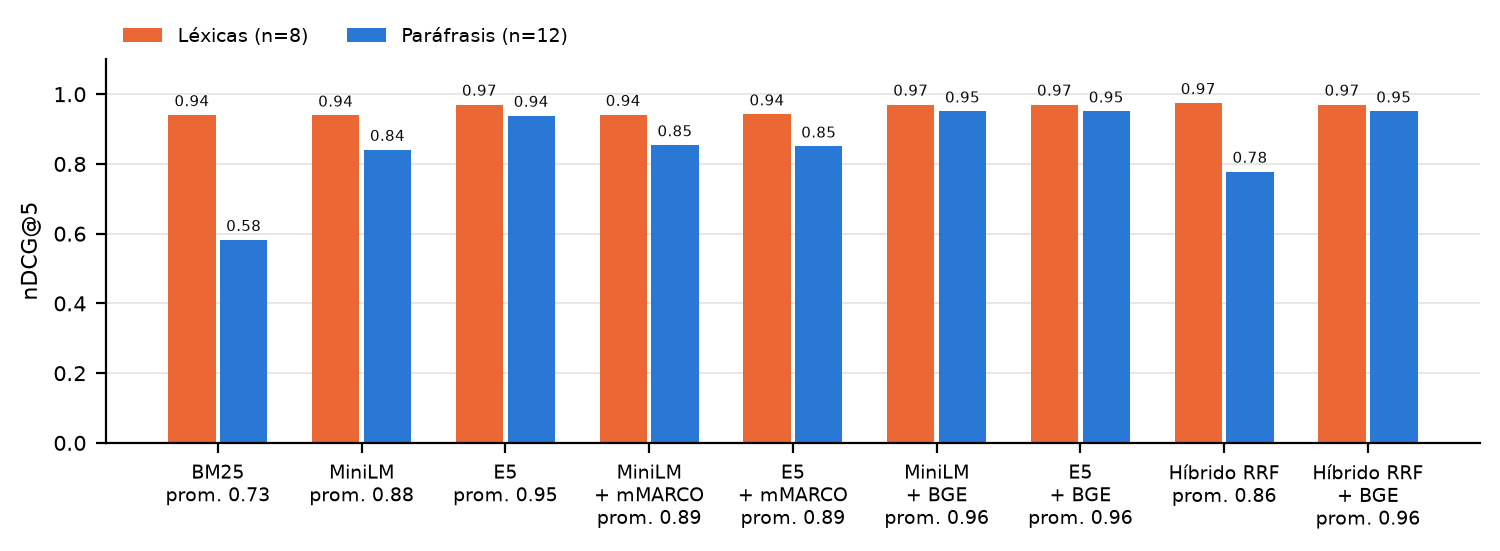
\includegraphics[width=0.93\linewidth]{ndcg_por_configuracion.png}
\caption{nDCG@5 por tipo de consulta. BM25 solo compite cuando consulta y documento comparten palabras.}
\end{figure}

\textbf{Lectura.} El salto lo da la representación densa. E5 sube el nDCG@5 de 0.725 a 0.951, y casi
todo el avance ocurre en paráfrasis (0.582 $\rightarrow$ 0.938). En consultas léxicas BM25 ya era bueno
y el semántico no lo empeora (0.940 $\rightarrow$ 0.970). E5 supera a BM25 en 13 consultas, empata en 5 y
pierde 2. E5 + BGE no pierde ninguna (14 victorias, 6 empates). Entre los dos \emph{embeddings}, E5 supera
a MiniLM (0.951 frente a 0.880; 9 victorias, 9 empates y 2 derrotas). El objetivo de entrenamiento pesa más
que la dimensión: E5 aprendió a emparejar consultas cortas con pasajes, mientras que MiniLM aprendió a
detectar frases equivalentes de longitud parecida. A cambio, E5 tarda $\approx$2.3$\times$ más en codificar cada consulta.

\section{Qué recupera el buscador semántico que el léxico ignoró por completo}

Criterio estricto: un documento relevante que \textbf{no recibe puntuación alguna de BM25} (no
comparte ni una raíz con la consulta y, por lo tanto, BM25 no lo ve a ninguna profundidad) y que
E5 + BGE coloca en su Top-5. Hubo \textbf{12 casos en 9 de las 20 consultas}
(\texttt{results/ejemplos\_semantico\_vs\_lexico.csv}). Cuatro de ellos muestran mecanismos distintos:

\begin{table}[H]
\centering\footnotesize
\begin{tabular}{@{}>{\raggedright\arraybackslash}p{2.9cm}>{\raggedright\arraybackslash}p{3.0cm}>{\raggedright\arraybackslash}p{4.3cm}>{\raggedright\arraybackslash}p{6.0cm}@{}}
\toprule
\textbf{Consulta} & \textbf{Raíces BM25 ($\mathit{df}$)} & \textbf{BM25, posición 1} & \textbf{E5 + BGE, posición 1 (y por qué)} \\
\midrule
\q{cita con el doctor por videollamada} & \term{cit}=2, \term{doctor}=0, \term{videollam}=0 &
\emph{Tenis y superficies de juego} (por «las grandes \emph{citas} del calendario»). nDCG@5 = 0.00 &
\emph{Telemedicina y consulta a distancia}: el texto dice «consulta remota por video» y
«especialista», no \emph{doctor} ni \emph{videollamada}. nDCG@5 = 1.00 \\
\addlinespace
\q{pan apto para celíacos} & \term{pan}=1, \term{apto}=0, \term{celiac}=0 &
\emph{El arte de la masa madre}, único resultado. nDCG@5 = 0.28 &
\emph{Panadería sin gluten}: el modelo asocia \emph{celíaco} con \emph{gluten} y \emph{trigo}, una
relación de conocimiento del mundo y no de sinonimia. nDCG@5 = 1.00 \\
\addlinespace
\q{cuidar el corazón} & \term{cuid}=0, \term{corazon}=1 &
\emph{Sushi y arroz avinagrado}, por «el \emph{corazón} del sushi…»: polisemia. nDCG@5 = 0.00 &
\emph{Dieta mediterránea} y \emph{Enfermedades cardiovasculares}: \emph{corazón} $\approx$
\emph{cardiovascular}, \emph{coronaria}, \emph{infarto}. nDCG@5 = 0.80 \\
\addlinespace
\q{vehículo de cero emisiones} & \term{vehicul}=4, \term{cer}=1, \term{emision}=3 &
\emph{Arquitectura de confianza cero} (ciberseguridad). nDCG@5 = 0.23 &
\emph{Automóviles eléctricos y autonomía}, aunque nunca dice \emph{cero emisiones}: E5 lo dejaba en la
posición 2 y BGE lo sube a la 1. nDCG@5 = 0.72 $\rightarrow$ 1.00 \\
\bottomrule
\end{tabular}
\end{table}

Los ejemplos muestran tres modos de fallo léxico distintos: \textbf{vocabulario ausente}
(\emph{doctor}, \emph{celíaco}: $\mathit{df}=0$), \textbf{polisemia} (\emph{corazón} del sushi) y
\textbf{coincidencia accidental} de una palabra frecuente (\emph{cita}, \emph{cero}). Los dos últimos son
peores que el primero porque BM25 responde con la misma seguridad que en un acierto, sin ninguna señal de
error. La recuperación densa los resuelve porque compara significados aprendidos de grandes corpus:
\emph{doctor}, \emph{médico} y \emph{especialista}, o \emph{celíaco} y \emph{gluten}, quedan cerca en el
espacio vectorial aunque no compartan letras. El caso inverso también ocurre. En \q{el derrumbe del
imperio de Roma}, BM25 acierta solo por \term{imperi}, la única raíz en común, porque la consulta dice
\emph{Roma} y el corpus dice \emph{romano}. Ese acierto depende de una sola raíz compartida.

\section{\emph{Re-ranking}: cuándo ayuda y cuánto cuesta}

\begin{figure}[H]
\centering
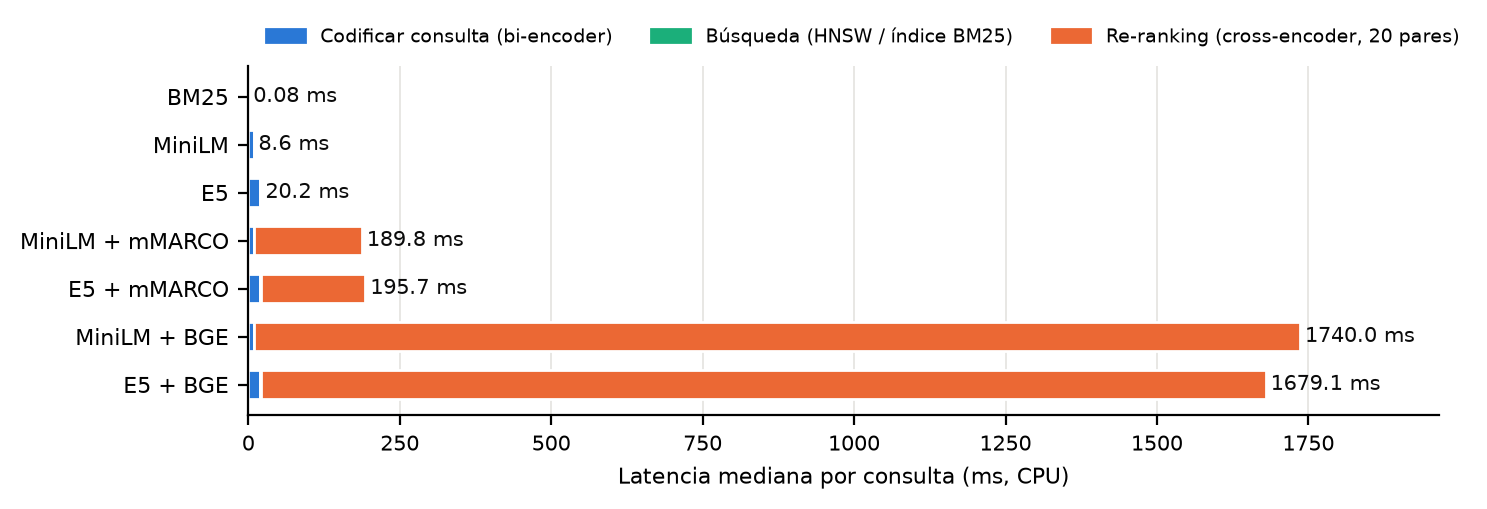
\includegraphics[width=0.86\linewidth]{latencias.png}
\caption{Latencia mediana por etapa (CPU). El \emph{re-ranking} domina el tiempo de cualquier pipeline que lo incluya.}
\end{figure}

\paragraph{La calidad depende del \emph{re-ranker}, no de tener dos etapas.} El \emph{cross-encoder}
ligero \textbf{empeoró} a E5 (0.951 $\rightarrow$ 0.887: 12 consultas peores y 2 mejores). En
\q{planetas parecidos a la Tierra donde podría haber vida} subió \emph{Exploración de Marte}, la Patagonia
y el Amazonas por encima de \emph{Exoplanetas y zonas habitables} (0.96 $\rightarrow$ 0.63): se aferró a
\emph{Tierra} y \emph{vida} en su sentido geográfico. BGE, 4.8$\times$ más grande, mejoró 8 consultas,
empató 8 y empeoró 4, hasta llegar a 0.959. Además corrigió \q{vehículo de cero emisiones}. Su peor caso fue
\q{cómo evitar que me roben las cuentas en internet} (0.83 $\rightarrow$ 0.66), donde puso \emph{Seguridad
en aplicaciones web} por encima de \emph{Phishing}. Como la primera etapa entrega casi todo lo relevante
(R@20 = 0.975; solo un documento de grado 1 de una consulta queda fuera en todos los sistemas), con BGE el orden final lo decide el
\emph{cross-encoder}: MiniLM + BGE, E5 + BGE e Híbrido + BGE obtienen el mismo nDCG@5 en las 20 consultas.

\paragraph{Latencia adicional.} La recuperación por coseno cuesta 20.2~ms con E5; el 99\,\% de ese tiempo
es codificar la consulta, porque HNSW responde en 0.13~ms. mMARCO añade 173~ms, $\approx$10$\times$
más lento, y BGE 1\,660~ms, \textbf{83$\times$}, con p95 de 1.95~s. Los tiempos absolutos variaron
hasta $\sim$50\,\% entre ejecuciones según la carga de la máquina; las proporciones se mantuvieron
estables ($\approx$10$\times$ y $\approx$80$\times$ en todas las corridas). El costo crece con el número de
candidatos, porque cada uno es una pasada completa del Transformer. Por eso el Top-20 es un compromiso:
más candidatos suben el techo de recall pero multiplican la latencia.

\paragraph{Fusión híbrida.} RRF(BM25, E5) es lo mejor en consultas léxicas (0.975), pero en paráfrasis
baja a 0.778. RRF da a BM25 el mismo voto aunque sus coincidencias sean accidentales: en \q{vehículo de
cero emisiones} reintroduce \emph{confianza cero} y el nDCG@5 cae a 0.33. Sin \emph{re-ranking},
conviene ponderar la fusión o activar BM25 solo con términos raros, como siglas, códigos o nombres propios,
que este corpus casi no tiene.

\section{Conclusión y recomendación}

La recuperación densa resuelve justo el límite que la actividad 2A dejó abierto: sinónimos,
paráfrasis y conocimiento implícito. Con E5, el nDCG@5 en paráfrasis pasa de 0.58 a 0.94 sin perder
calidad en las consultas léxicas. La segunda etapa solo mejora si el \emph{cross-encoder} es mejor juez
que el \emph{bi-encoder}. Con BGE se gana 0.008 de nDCG@5 a cambio de $\approx$1.7~s por consulta en CPU;
con mMARCO se pierde calidad y además se paga latencia.
\textbf{Recomendación:} para búsqueda interactiva, \textbf{E5 solo} (0.951 en $\approx$20~ms: 99\,\% de
la calidad con $\sim$1\,\% del tiempo). Para la etapa de recuperación de un RAG, donde un segundo extra es
tolerable, \textbf{E5 + BGE}, idealmente en GPU, donde el \emph{re-ranking} cuesta uno o dos órdenes de
magnitud menos.
\textbf{Limitaciones:} 20 consultas y 120 documentos, con diferencias de centésimas que no son
significativas. Los juicios los asignó una sola persona. BGE se añadió \emph{después} de ver que mMARCO
empeoraba los resultados, así que su ventaja no está validada en un conjunto independiente.

\end{document}
